\documentclass[journal,twocolumn]{IEEEtran}
\usepackage{graphicx}
\graphicspath{{figures/}}
\DeclareGraphicsExtensions{.pdf,.jpeg,.png}
\usepackage{amsmath}
\usepackage{float}
\usepackage{url}
\usepackage{hyperref}
\usepackage[T1]{fontenc}
\usepackage[utf8]{inputenc}
\usepackage{authblk}
\usepackage{physics}
\hyphenation{op-tical net-works semi-conduc-tor}
\usepackage[sorting=none, backend=bibtex]{biblatex}
\nocite{*}
\addbibresource{references}

\begin{document}

\title{Shallow-learning methods for pedestrian classification and detection in images}

\author[1]{Master’s degree in Computer Engineering for Robotics and Smart Industry\\Machine Learning and Artificial Intelligence course, a.a. 2021/2022\\ Lorenzo Busellato}%
\affil[1]{VR472249, lorenzo.busellato\_02@studenti.univr.it}
\onecolumn

\maketitle
\begin{abstract} Pedestrian detection is a key task in the computer vision field, given its obvious applications in surveillance systems, autonomous driving and robotics. 
This work presents a pipeline for shallow-learning based pedestrian detection. The Histogram of Oriented Gradients (HOG)
method for feature extraction is described and applied to the Daimler Mono Pedestrian Classification Benchmark Data Set. Three classification
techniques, Support Vector Machines (SVMs), K-Nearest Neighbors (KNN) and Naive Bayes, are described and benchmarked
with different sets of hyperparameters. The benchmarks are then compared against each other to determine the best performing
method in terms of accuracy in classification. Finally the best performing method is used to implement a full pedestrian detection pipeline.
\end{abstract}
  \tableofcontents
  \listoffigures
  \listoftables  
  \clearpage
  \twocolumn

\IEEEpeerreviewmaketitle

\section{Introduction}
\IEEEPARstart{T}{he} task of pedestrian detection, i.e. the task of localizing pedestrians within an image, is one of the most tackled
instances of the broader class of object detection problems.
This is due to its natural applications in autonomous driving,
surveillance and robotics. For instance, in the US alone about
5000 of the 35000 annual car accident fatalities involve
pedestrians \cite{1}, therefore the need for automated methods for
pedestrian detection is apparent.

The task of pedestrian detection presents a series of complexities regarding the high variability in scale and size of the
person within the image, occlusions with the rest of the scene,
susceptibility to lighting conditions and the real time detection
requirement.

The main models that are used for pedestrian detection are
hand-crafted models and deep learning models. Hand-crafted
models are based on classification of hand-crafted features. Deep learning models on the other hand typically use
convolutional neural networks for the extraction of features,
therefore producing high-level semantic representations of
objects.
In this work the first class of models will be analyzed
and implemented. Specifically, the Histogram of Oriented
Gradients (HOG) method will be used to extract features from
images, because it is known\cite{2} that it is the best performing non-deep learning based feature extractor for human detection. The classification of images will then be implemented
using non-deep learning methods, namely Support Vector
Machines (SVMs), K-Nearest Neighbors (KNN) and Naive Bayes. Finally the best performing classifier will be used
to implement a pedestrian detector.

The main objectives of this work are described in section
\ref{sec:obj}. The data set and methodology employed are described in
sections \ref{sec:data} and \ref{sec:meth}. The experimental evaluation is presented
in section \ref{sec:exp}. The conclusions are summarized in section \ref{sec:conc}.

\section{Objectives}
\label{sec:obj}
The main objective of this work is the implementation of
a pedestrian detection pipeline, which is made up
of three main components: a feature extractor, a classifier and a
detector.

Regarding the classifiers, the objective is to obtain an in-depth comparison between the performance of some well-known shallow learning techniques with respect to the problem of pedestrian detection, as well as the relation between hyperparameters and classifier performance.

Finally, the best performing classifier will be used to implement a detector, therefore completing the pedestrian detection pipeline. The pipeline will then be applied to a video sequence in order to showcase its performance.

\section{Dataset}
\label{sec:data}

The data set used in this work is the Daimler Mono Pedestrian Classification Benchmark Data Set. The data set consists of four separate subsets: the base set and three additional sets. The base set is divided into five subsets, three for training (named "1", "2" and "3") and two for testing (named "T1" and "T2"). All five sets contain 4800 18$\times$36 grayscale images containing pedestrians and 5000 18$\times$36 grayscale images not containing pedestrians. The three additional sets each contain 1200 640$\times$280 grayscale images for the purpose of extracting additional negative samples for the hard-negative mining procedure.

\begin{figure}[h]
\begin{minipage}{0.45\columnwidth}
\centering
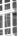
\includegraphics[keepaspectratio,width=0.4\textwidth]{1}
\end{minipage}
\begin{minipage}{0.45\columnwidth}
\centering
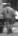
\includegraphics[keepaspectratio,width=0.4\textwidth]{2}
\end{minipage}
\caption[Example images from the dataset]{Example figures from the training data set. On the left a non-pedestrian sample, on the right a pedestrian sample.}
\end{figure}

In this work, data sets 1, 2 and 3 will be grouped together in a singular data set for the training of the models, as will data sets T1 and T2 for the testing.

\section{Methodology}
\label{sec:meth}

\subsection{Histogram of Oriented Gradients}

Given an input image $I$, for each pixel $(x,y)\in I$ the gradients $G_x$ and $G_y$ are computed. This is typically done via a convolution operation:

\begin{equation}
G_x=\omega_x* I\;\;\;\;\;G_y=\omega_y* I
\end{equation}

where $\omega_x$ and $\omega_y$ are the kernels associated to the convolution operation. The most common kernels used in the context of pedestrian detection are:

\begin{equation*}
\omega_x=\begin{bmatrix}
-1 & 0 & 1
\end{bmatrix}\;\;\;\;\;\omega_y=\omega_x^T
\end{equation*}

They are the most commonly used because experimentally it is observed\cite{2} that they produce the least amount of detected false positives per moving window (FFPW) compared to other kernels.

After the convolution operation, two gradient matrices are obtained, $G_x$ and $G_y$. For each pixel $(x,y)\in I$ then the magnitude $\mu$ and angle $\theta$ are computed:

\begin{equation}
\mu(i,j)=\sqrt{G_x(i,j)^2+G_y(i,j)^2}
\end{equation}

\begin{equation*}
\theta(i,j)=\abs{\tan^{-1}\left(\frac{G_y(i,j)}{G_x(i,j)}\right)}
\end{equation*}

In practice the angle is computed with $atan2$, therefore it is in the range $(\pi,\pi]$.

The resulting gradient magnitude and gradient angle matri-
ces are then divided into $8\times 8$ patches, for each of which a 9-point histogram of oriented gradients is computed. A
histogram is a series of bins labeled with angle values. The
number of bins is determined by the angle step between
the bins, for instance with an angle step of 20 degrees the
histogram will have $180^\circ/20^\circ = 9$ bins.

For each pixel in the patch, the corresponding gradient angle
determines two bins on the histogram that the pixel votes for.
The two bins selected are those which represent the two closest
angles to the given gradient angle value. The value added to
the selected bins is proportional to the distance of the gradient
angle to the bin angle, the gradient magnitude and the step
between the bins:
\begin{equation*}
v_{closest}=\frac{(binAngle-\theta)\mu}{angleStep}
\end{equation*}
\begin{equation*}
v_{2nd-closest}=\frac{(\theta-binAngle)\mu}{angleStep}
\end{equation*}

Repeating the process for each 8 × 8 patch, a 16$\times$8 matrix
of histograms is constructed.
To reduce the variability in gradient intensities due to lighting conditions and foreground-background contrast, a block
normalization procedure is introduced. The 16$\times$8 histogram
matrix is scanned with a 2$\times$2 window producing 15$\times$7 blocks,
for each of which a normalized histogram vector is computed
by concatenating the four histograms contained in the block
and normalizing the resulting vector.
Finally, the feature descriptor for the image is constructed
by concatenating the normalized histogram vectors. From
each 8$\times$8 patch a 1$\times$9 vector is collected, which is then
concatenated with another three 1$\times$9 vectors composing a
1$\times$36 vector, which is finally concatenated with another
fourteen 1$\times$36 vectors, resulting in a 1$\times$3780 feature vector.

\begin{figure}[h]
\centering
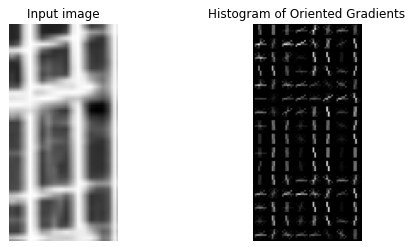
\includegraphics[keepaspectratio,width=0.9\columnwidth]{3}
\caption[HOG representation of a non-pedestrian sample]{Histogram of Oriented Gradients representation of a non-pedestrian sample.}
\label{fig:3}
\end{figure}
\begin{figure}[h]
\centering
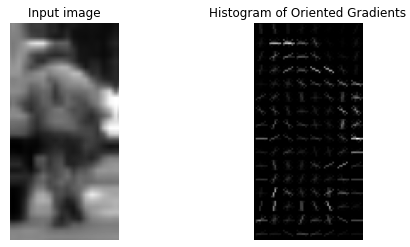
\includegraphics[keepaspectratio,width=0.9\columnwidth]{4}
\caption[HOG representation of a pedestrian sample]{Histogram of Oriented Gradients representation of a pedestrian sample.}
\label{fig:4}
\end{figure}

A representation of the resulting feature vector can be seen in figures \ref{fig:3} and \ref{fig:4}. The representation is obtained by plotting the 9$\times$1 normalized histograms in each 8$\times$8 cell. The dominant direction of the histogram is able to capture contours, especially straight lines such as the frame of the window in figure \ref{fig:3} or the legs of the pedestrian in figure \ref{fig:4}. The gradient magnitudes also carry information on the lighting of the scene, with greater magnitudes corresponding to lighter areas.

\subsection{Naive Bayes}

\subsection{K-Nearest Neighbors}

\subsection{Support Vector Machine}

\subsection{Hard-negative mining}

\subsection{Pedestrian detection}

\subsection{Non-maximum suppression}

\section{Experiments and results}
\label{sec:exp}

\subsection{Adopted metrics}

\subsection{Performed experiments}

\subsection{Results}

\section{Conclusions}
\label{sec:conc}

\printbibliography


\end{document}